
  \begin{center}
    \normalsize{\cyr{\textbf{№3.1}}}
  \end{center}

  \begin{figure}[h!]
    \centering
    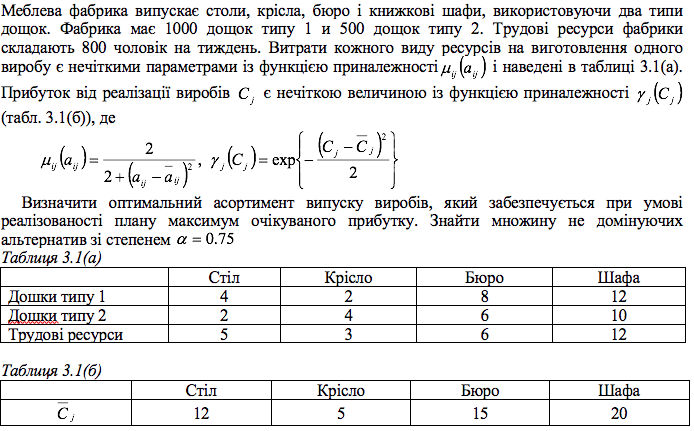
\includegraphics[width=14cm]{3_1.png}
    \centering
  \end{figure}

Математична модель: $x_{j}$ продукт $j$
\Code{
max \quad   \sum_j^4\  C_{j} x_{j} \qquad  \text{Обмеження} \quad  \sum_{j=1}^3 a_{ij}  x_{j} \leqslant b_j
}

\begin{multicols}{2}
  $$\mu(a_{ij}) \geqslant 0.75  $$

  $$\dfrac{2}{2+(a_{ij}-\overline{a}_{ij})^2} \geqslant 0.75$$
  $$\dfrac{2}{0.75} \geqslant 2+(a_{ij}-\overline{a}_{ij})^2$$
  $$\dfrac{2}{0.75} - 2 \geqslant (a_{ij}-\overline{a}_{ij})^2$$
  $$\dfrac{2}{3} \geqslant (a_{ij}-\overline{a}_{ij})^2$$
  $$ \sqrt{\dfrac{2}{3}} \geqslant |a_{ij}-\overline{a}_{ij}|$$
  $$ a_{ij} - \sqrt{\dfrac{2}{3}} \leqslant a_{ij} \leqslant a_{ij} + \sqrt{\dfrac{2}{3}}$$

  \columnbreak

  $$\gamma(C_{ij}) \geqslant 0.75 $$

  $$\exp\{ - \dfrac{(C_{ij}-\overline{C}_{ij})^2}{2} \} \geqslant 0.75 $$
  $$- \dfrac{(C_{ij}-\overline{C}_{ij})^2}{2} \geqslant \ln{0.75} $$
  $$ (C_{ij}-\overline{C}_{ij})^2 \leqslant -2 \ln{0.75} $$
  $$ (C_{ij}-\overline{C}_{ij})^2 \leqslant 2 \ln{\dfrac{1}{0.75}} $$
  $$|C_{ij}-\overline{C}_{ij}| \leqslant \sqrt{2\ln{\dfrac{4}{3}}} $$
  $$ \overline{C}_{ij} - \sqrt{2 \ln{\dfrac{4}{3}}} \leqslant C_{ij} \leqslant \overline{C}_{ij} + \sqrt{ 2 \ln{\dfrac{4}{3}}}$$

\end{multicols}

\begin{multicols}{2}

  \Title{Задача песиміста}
  \Code{
    max \quad \sum_{j=1}^4( \overline{C}_{j} - \sqrt{ 2 \ln{\dfrac{4}{3}}} ) x_{j}
  }

  \Title{Обмеження}
  \Code{
    \sum_{i=1}^3( a_{ij} + \sqrt{\dfrac{2}{3}} ) x_{j} \leqslant b_i
  }

  \columnbreak

  \Title{Задача оптиміста}
  \Code{
    max \quad \sum_{j=1}^4( \overline{C}_{j} + \sqrt{ 2 \ln{\dfrac{4}{3}}} ) x_{j}
  }

  \Title{Обмеження}
  \Code{
    \sum_{i=1}^3( a_{ij}  - \sqrt{\dfrac{2}{3}} ) x_{j} \leqslant b_i
  }

\end{multicols}
